\section{Model fitting} \label{sec:ModelFitting}
In the following section we try to find and determine a model to describe the evolution of the done status of the nodes as a function of time elapsed. Given the shape shown in Figure \ref{fig:done-status} there are several options that might fit the general trend of the curve:

\begin{itemize}
	\item Logistic model $ Y = \frac{A}{1 + e^{-Rt}} $
	\item Variation of the logistic model $ Y = A\frac{1-e^{-Rt}}{1+e^{-Rt}}$
	\item Gompertz model $ Y = Ae^{-Be^{-Rt}} $
	
	\item Asymptotic model $ Y = A + Be^{-Rt}$
\end{itemize} 

The next step is to find the most adapt for our case: by looking at the requirements and assumptions of each model, some of them need to be excluded. The first one is quickly discarded because it is more fit to describe the probability of success for a given case, even though the curves between the model and the time evolution of the system look similar, it would be wrong to use the equation improperly.
The asymptotic model is discarded because its second derivative has no change in sign, this is not applicable to the system because, as show in Figure \ref{fig:done-status} the function can have a change in curvature.


Both Gompertz and the variation for the logistic model (not really the variation, but one of them) are used to represent "growth of population" dynamics and could adapt to the system case, but some checks need to be done before proceeding any further.

By performing a residual analysis the Gompertz model results to be the most suited for our samples i. e. for the configuration of $p=0.15$  $r=10$ the MSE value for Gompertz is 0,0027 meanwhile the one for the variation is 0,2984. Note that these values are very close to 0 since a spreadsheet solver was used to minimize the MSE (with the found values $A=0.9117$ $B=4.0959$ and $R=0.0414$), a QQ plot for this configuration is shown below. In addition the use of the Gompertz model fits the logic of one of its typical case: examining diseases spread. Regarding the variation of the logistic model the value generated by the solver were $A=0.9474$ and $R=0.0264$


\begin{figure}[H]
    \centering
    \subfloat[\centering Gompertz model]{{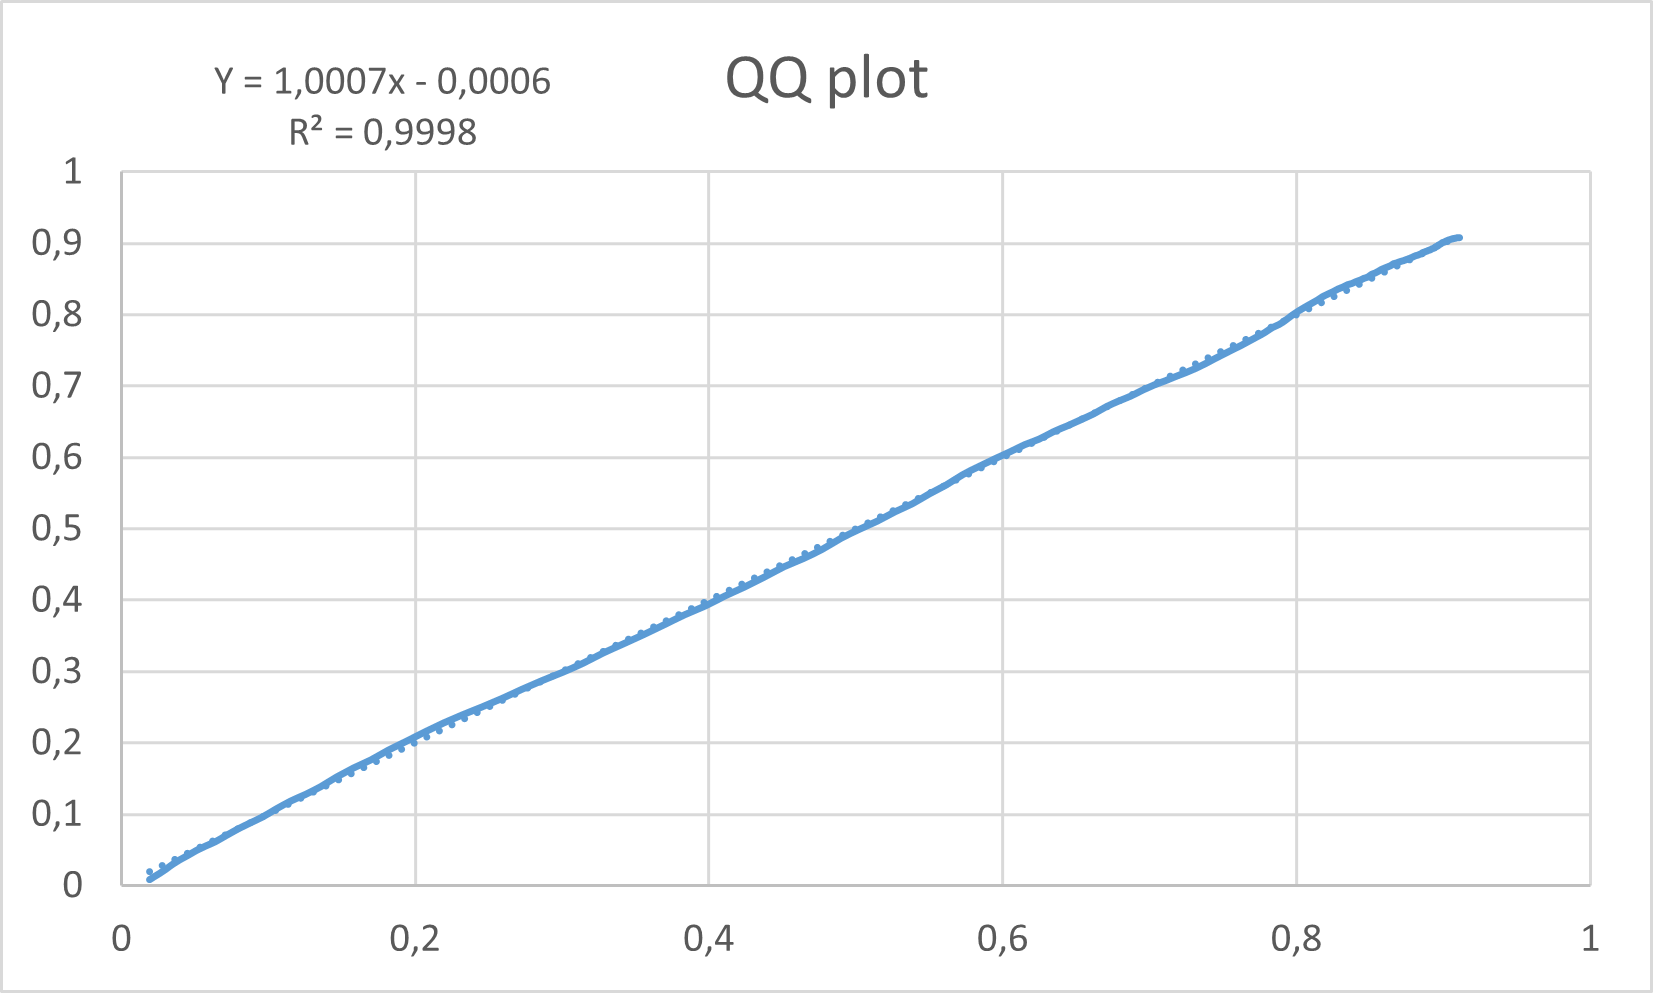
\includegraphics[width=8cm]{./images/QQPlot200.png} }}
    \qquad
    \subfloat[\centering Variation of the logistic model]{{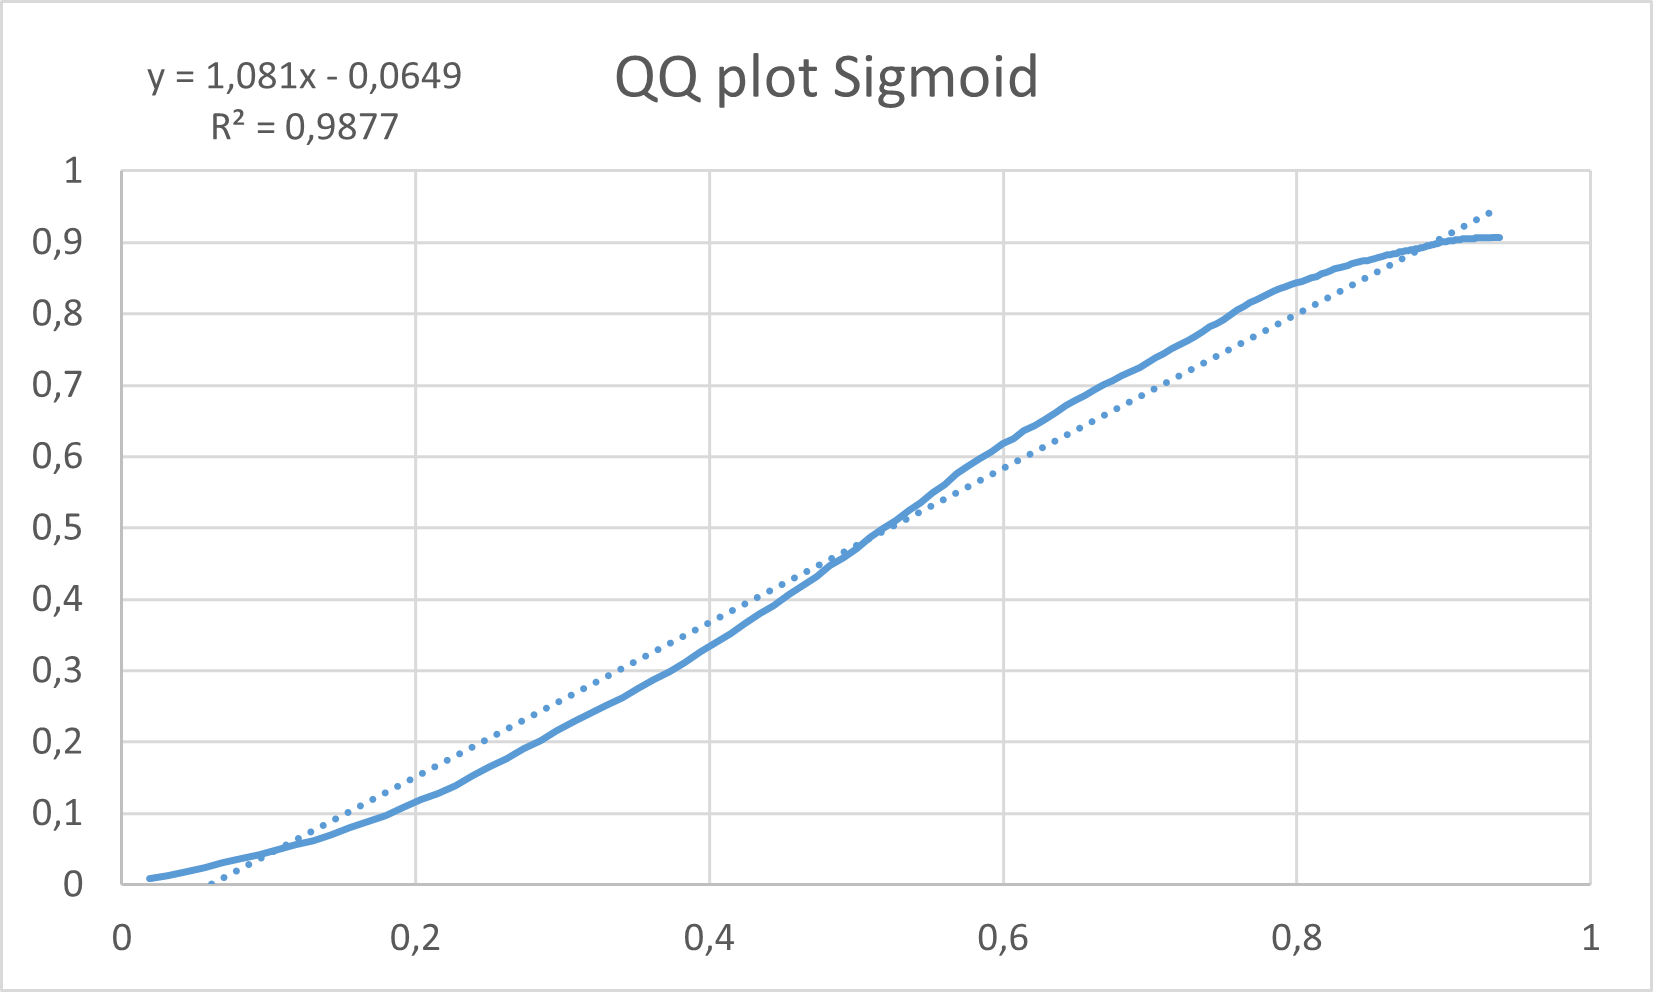
\includegraphics[width=8cm]{./images/QQPlotSigmoid200.png}}}
    \caption{QQ plots for the models}
\end{figure}




The QQ plot confirms linear relationship between the values from our sample and the ones from the Gompertz model, this is also indicated by the value for $R^2$.

\section{Factorial analysis on the models parameters}
As previously stated we consider for extremes the values 0.15 and 0.85 for probability and 10 and 75 for the radius.

The Gompertz model ($ Y = Ae^{-Be^{-Rt}} $) has three parameters:
\begin{itemize}
	\item A is the asymptote
	\item B is the displacement on the x axis
	\item R is the grow rate
\end{itemize}
The first to be analyzed is the asymptote.

\begin{table}[H]
\centering
\begin{tabular}{|cc|cc|}
\hline
\multicolumn{2}{|c|}{\multirow{2}{*}{\textbf{Asymptote}}} & \multicolumn{2}{c|}{\textbf{Radius}} \\ \cline{3-4} 
\multicolumn{2}{|c|}{} & \multicolumn{1}{c|}{\textbf{10}} & \textbf{75} \\ \hline
\multicolumn{1}{|c|}{\multirow{2}{*}{\textbf{Probability}}} & \textbf{15} & \multicolumn{1}{c|}{0,9117} & 0,9995 \\ \cline{2-4} 
\multicolumn{1}{|c|}{} & \textbf{85} & \multicolumn{1}{c|}{0,5741} & 0,9185 \\ \hline
\end{tabular}
\caption{Extreme factor levels for asymptote}
\end{table}

\begin{table}[H]
\centering
\begin{tabular}{c|c|c|c|c|cc}
\cline{2-7}
 & \textbf{I} & \textbf{Probability} & \textbf{Radius} & \textbf{Combined} & \multicolumn{1}{c|}{\textbf{Asymptote}} & \multicolumn{1}{c|}{\textbf{SD\_i}} \\ \cline{2-7} 
 & 1 & -1 & -1 & 1 & \multicolumn{1}{c|}{0,9117} & \multicolumn{1}{c|}{0,0037} \\ \cline{2-7} 
 & 1 & 1 & -1 & -1 & \multicolumn{1}{c|}{0,5741} & \multicolumn{1}{c|}{0,0766} \\ \cline{2-7} 
 & 1 & -1 & 1 & -1 & \multicolumn{1}{c|}{0,9995} & \multicolumn{1}{c|}{0,0221} \\ \cline{2-7} 
 & 1 & 1 & 1 & 1 & \multicolumn{1}{c|}{0,9185} & \multicolumn{1}{c|}{0,0046} \\ \hline
\multicolumn{1}{|c|}{\textbf{4q}} & 3,4037 & -0,4185 & 0,4322 & 0,2565 & \multicolumn{1}{c|}{Total} & \multicolumn{1}{c|}{0,1069} \\ \hline
\multicolumn{1}{|c|}{\textbf{q}} & 0,8509 & -0,1046 & 0,1080 & 0,0641 &  &  \\ \cline{1-5}
\multicolumn{1}{|c|}{\textbf{4 q\textasciicircum{}2}} &  & 0,0438 & 0,0467 & 0,0165 &  &  \\ \cline{1-5}
\multicolumn{1}{|c|}{\textbf{Influence}} &  & 0,4095 & 0,4366 & 0,1539 &  &  \\ \cline{1-5}
\end{tabular}
\caption{Influence of factors for asymptote}
\end{table}

We then follow with the tables for displacement.

\begin{table}[H]
\centering
\begin{tabular}{|cc|cc|}
\hline
\multicolumn{2}{|c|}{\multirow{2}{*}{\textbf{Displacement}}} & \multicolumn{2}{c|}{\textbf{Radius}} \\ \cline{3-4} 
\multicolumn{2}{|c|}{} & \multicolumn{1}{c|}{\textbf{10}} & \textbf{75} \\ \hline
\multicolumn{1}{|c|}{\multirow{2}{*}{\textbf{Probability}}} & \textbf{15} & \multicolumn{1}{c|}{4,0959} & 1,8622 \\ \cline{2-4} 
\multicolumn{1}{|c|}{} & \textbf{85} & \multicolumn{1}{c|}{3,8693} & 0,5905 \\ \hline
\end{tabular}
\caption{Extreme factor levels for displacement}
\end{table}

\begin{table}[H]\label{tab:InflDisp}
\centering
\begin{tabular}{c|c|c|c|c|cc}
\cline{2-7}
 & \textbf{I} & \textbf{Probability} & \textbf{Radius} & \textbf{Combined} & \multicolumn{1}{c|}{\textbf{Displacement}} & \multicolumn{1}{c|}{\textbf{SD\_i}} \\ \cline{2-7} 
 & 1 & -1 & -1 & 1 & \multicolumn{1}{c|}{4,0959} & \multicolumn{1}{c|}{2,2243} \\ \cline{2-7} 
 & 1 & 1 & -1 & -1 & \multicolumn{1}{c|}{3,8693} & \multicolumn{1}{c|}{1,5999} \\ \cline{2-7} 
 & 1 & -1 & 1 & -1 & \multicolumn{1}{c|}{1,8622} & \multicolumn{1}{c|}{0,5509} \\ \cline{2-7} 
 & 1 & 1 & 1 & 1 & \multicolumn{1}{c|}{0,5905} & \multicolumn{1}{c|}{4,0563} \\ \hline
\multicolumn{1}{|c|}{\textbf{4q}} & 10,4179 & -1,4983 & -5,5125 & -1,0453 & \multicolumn{1}{c|}{Total} & \multicolumn{1}{c|}{8,4314} \\ \hline
\multicolumn{1}{|c|}{\textbf{q}} & 2,6045 & -0,3746 & -1,3781 & -0,2613 &  &  \\ \cline{1-5}
\multicolumn{1}{|c|}{\textbf{4 q\textasciicircum{}2}} &  & 0,5612 & 7,5970 & 0,2731 &  &  \\ \cline{1-5}
\multicolumn{1}{|c|}{\textbf{Influence}} &  & 0,0666 & 0,9010 & 0,0324 &  &  \\ \cline{1-5}
\end{tabular}
\caption{Influence of factors for displacement}
\end{table}

Finally we end up with the tables for the growth rate.

\begin{table}[H]
\centering
\begin{tabular}{|cc|cc|}
\hline
\multicolumn{2}{|c|}{\multirow{2}{*}{\textbf{Grow Rate}}} & \multicolumn{2}{c|}{\textbf{Radius}} \\ \cline{3-4} 
\multicolumn{2}{|c|}{} & \multicolumn{1}{c|}{\textbf{10}} & \textbf{75} \\ \hline
\multicolumn{1}{|c|}{\multirow{2}{*}{\textbf{Probability}}} & \textbf{15} & \multicolumn{1}{c|}{0,0414} & 0,1283 \\ \cline{2-4} 
\multicolumn{1}{|c|}{} & \textbf{85} & \multicolumn{1}{c|}{0,1595} & 0,3660 \\ \hline
\end{tabular}
\caption{Extreme factor levels for growth rate}
\end{table}


\begin{table}[H]
\centering
\begin{tabular}{c|c|c|c|c|cc}
\cline{2-7}
 & \textbf{I} & \textbf{Probability} & \textbf{Radius} & \textbf{Combined} & \multicolumn{1}{c|}{\textbf{Growth}} & \multicolumn{1}{c|}{\textbf{SD\_i}} \\ \cline{2-7} 
 & 1 & -1 & -1 & 1 & \multicolumn{1}{c|}{0,0414} & \multicolumn{1}{c|}{0,0175} \\ \cline{2-7} 
 & 1 & 1 & -1 & -1 & \multicolumn{1}{c|}{0,1595} & \multicolumn{1}{c|}{0,0002} \\ \cline{2-7} 
 & 1 & -1 & 1 & -1 & \multicolumn{1}{c|}{0,1283} & \multicolumn{1}{c|}{0,0021} \\ \cline{2-7} 
 & 1 & 1 & 1 & 1 & \multicolumn{1}{c|}{0,3660} & \multicolumn{1}{c|}{0,0369} \\ \hline
\multicolumn{1}{|c|}{\textbf{4q}} & 0,6952 & 0,3558 & 0,2933 & 0,1197 & \multicolumn{1}{c|}{Total} & \multicolumn{1}{c|}{0,0567} \\ \hline
\multicolumn{1}{|c|}{\textbf{q}} & 0,1738 & 0,0890 & 0,0733 & 0,0299 &  &  \\ \cline{1-5}
\multicolumn{1}{|c|}{\textbf{4 q\textasciicircum{}2}} &  & 0,0317 & 0,0215 & 0,0036 &  &  \\ \cline{1-5}
\multicolumn{1}{|c|}{\textbf{Influenza}} &  & 0,5578 & 0,3791 & 0,0631 &  &  \\ \cline{1-5}
\end{tabular}
\caption{Influence of factors for growth rate}
\end{table}


These results confirm our initial ideas and expectations: the first thing to notice is that the influences for the asymptote are similar to the ones for the coverage percentage; this make sense because the asymptote is the maximum height of the curve and the coverage percentage is the maximum coverage that a run achieves, so it's natural for them to be almost the same. 

\medskip
The displacement represent how high is the percentage of nodes in the done status at the second clock of each run, the first one is excluded because it's always constant due to the fact that at the first clock only the zero-patient node is done. By translating these results on the actual model for the analysis, the displacement represent how well the firstly infected node is connected and how many of its neighbors immediately pass the RV threshold for sending a new infection message. It make sense for the radius to have 90\% influence because having a big radius means having a lot of neighbors. Pay attention that the q values in Table \ref{tab:InflDisp} are negative so, by incrementing the radius, we are diminishing the displacement; this makes sense since lower values for the B parameter indicates a higher Y(t) when t = 0 in the Gompertz function. A low displacement is not always a good thing however because a big radius, as previously shown, can lead to more collision and less coverage percentage in some cases. 

\medskip
In regards of the analysis a high growth rate is achieved when nodes do not experience many collisions and thus, after receiving a message correctly, can quickly relay it. So it make sense for the probability to influence the 55\% of the result. The radius accounts for a little more the a third of the influence: this is easy to imagine since a high radius means a high number of nodes reached.

\medskip
These results give us a general idea on how the factors weight on the model and how to maximize certain aspects of it, but to perform a proper analysis of the system it is a good idea to pair these values with the box-plot and factorial analysis previously presented.